% MUSCAT Framework Paper - IEEE/AIAA DASC Format
% Enhanced Multi-Sensor Optimization for C-UAS using Genetic Algorithms

\documentclass[conference]{IEEEtran}

% Packages
\usepackage{cite}
\usepackage{amsmath,amssymb,amsfonts}
\usepackage{algorithmic}
\usepackage{graphicx}
\usepackage{textcomp}
\usepackage{xcolor}
\usepackage{booktabs}
\usepackage{multirow}
\usepackage{url}
\usepackage{hyperref}

% Custom commands
\newcommand{\mc}{M_c}
\newcommand{\mg}{M_g}
\newcommand{\pnet}{\bar{P}_{Net}}
\newcommand{\rnet}{\bar{R}}

\begin{document}

% Title
\title{Scalable Multi-Objective Optimization for Urban BVLOS Surveillance Infrastructure Planning}

% Authors
\author{
\IEEEauthorblockN{Your Name\IEEEauthorrefmark{1}, Co-Author Name\IEEEauthorrefmark{2}}
\IEEEauthorblockA{\IEEEauthorrefmark{1}Your Institution, Department\\
City, Country\\
Email: your.email@institution.edu}
\IEEEauthorblockA{\IEEEauthorrefmark{2}Co-Author Institution\\
Email: coauthor@institution.edu}
}

\maketitle

% Abstract
\begin{abstract}
The safe integration of Beyond Visual Line of Sight (BVLOS) operations and Urban Air Mobility (UAM) into dense urban airspace requires robust Ground-Based Surveillance Systems (GBSS), yet no existing framework addresses the simultaneous challenges of high-fidelity urban modeling, multi-objective optimization, and real-world validation at city scale. This paper presents a holistic methodology that integrates four key components: (1) OpenStreetMap for automatic acquisition of building geometries from any city worldwide, (2) deterministic 3D ray-tracing for accurate line-of-sight calculations with urban obstacles, (3) multi-objective optimization via NSGA-II to discover Pareto-optimal trade-offs between coverage, redundancy, and cost, and (4) scalable Genetic Algorithms enabling optimization of networks with 50-100 sensor locations—previously intractable. The framework optimizes heterogeneous sensor networks (Radar, RF, Electro-Optical, Acoustic) discovering a continuum of non-dominated solutions rather than prescribing a single configuration, enabling infrastructure selection based on operational context and risk profiles. Real-world validation with São Paulo's Avenida Paulista (4,921 buildings over 2.94 km²) represents the largest urban C-UAS placement study in literature—50x larger than prior work—demonstrating global applicability and providing the first computationally viable tool for prescriptive UTM infrastructure planning at city scale. Results maintain full compatibility with MUSCAT metrics, facilitating regulatory adoption.
\end{abstract}

% Keywords
\begin{IEEEkeywords}
Beyond Visual Line of Sight (BVLOS), Urban Air Mobility (UAM), Ground-Based Surveillance Systems (GBSS), Detect-and-Avoid (DAA), UTM infrastructure, Multi-sensor optimization, Genetic algorithms, OpenStreetMap, Urban environment modeling
\end{IEEEkeywords}

% Sections
% Section 1: Introduction

\section{Introduction}

\subsection{Enabling Safe BVLOS and UAM Operations}

The rapid growth of Beyond Visual Line of Sight (BVLOS) drone operations and Urban Air Mobility (UAM) promises transformative economic benefits, from autonomous package delivery to air taxis \cite{faa2023uam}. However, safe integration into dense urban airspace requires addressing a critical infrastructure gap: continuous, reliable surveillance coverage to enable Detect-and-Avoid (DAA) capabilities for all aircraft, both manned and unmanned \cite{mueller2017enabling}.

Unlike traditional Air Traffic Control (ATC) systems that rely on cooperative transponders, future UTM (UAS Traffic Management) architectures must detect \textit{all} airspace users—including non-cooperative or malfunctioning drones—to prevent collisions and ensure public safety \cite{faa2020utm}. This surveillance requirement directly impacts airspace capacity: regulators mandate larger separation "bubbles" (e.g., 500m radius) when surveillance is uncertain, drastically reducing the number of concurrent operations possible in a urban corridor \cite{nasa2021utm}. Conversely, high-confidence surveillance enables tighter separations (e.g., 50m), increasing corridor capacity by orders of magnitude.

\subsection{Ground-Based Surveillance Systems (GBSS)}

Ground-Based Surveillance Systems (GBSS) provide the foundational surveillance layer for UTM, complementing aircraft-based DAA sensors by offering persistent, infrastructure-supported coverage \cite{kopardekar2016unmanned}. However, no single sensor technology can reliably detect all airspace users in urban environments due to inherent physical limitations: radars provide all-weather detection but have short ranges for small RCS targets; RF/RID receivers are cost-effective but depend on cooperative emitters; electro-optical sensors lack range in adverse weather; acoustic sensors suffer from urban noise \cite{guvenc2018detection}.

This technological diversity necessitates \textit{heterogeneous} multi-sensor networks that fuse complementary capabilities to achieve the coverage reliability and redundancy required by UTM. The resulting GBSS also serves dual-purpose security functions (Counter-UAS detection of unauthorized drones), further motivating infrastructure investment. However, designing cost-effective GBSS deployments presents a formidable optimization challenge: determining the optimal number, types, and spatial placement of sensors to maximize coverage and resilience across square-kilometer urban areas while satisfying budget constraints and physical deployment constraints (building rooftops, towers, etc.).

\subsection{Prior Work and Remaining Challenges}

Kukulka de Albuquerque et al. \cite{muscat2023} addressed this challenge with MUSCAT (Mason's UAV Systems and Cyber Analysis Testbed), a framework combining JDL Data Fusion principles with systems engineering for sensor placement optimization. Their methodology established rigorous metrics (Coverage Index $\mc$, Gap Index $\mg$, Cost-Effectiveness $CA$) and demonstrated effectiveness for corridor design using terrain elevation models (DTED) and exhaustive enumeration of sensor combinations. However, their exhaustive search approach—while optimal for small scenarios—faces fundamental scalability limits that prevent application to real urban deployments, as detailed below.

\subsection{Research Gaps in Current Approaches}

Despite advances in C-UAS sensor network design, three critical gaps remain unaddressed in the literature:

\textbf{Gap 1 - Scalability}: Most optimization approaches suffer from computational intractability for realistic urban scenarios. Exhaustive search methods \cite{muscat2023} evaluate all combinations resulting in $O(2^n)$ complexity—infeasible beyond 10-15 potential positions. Mixed-Integer Programming formulations \cite{aievola2022ground} face similar NP-hard scaling challenges. For urban C-UAS deployment requiring 50-100 sensors across several square kilometers, these approaches become computationally prohibitive.

\textbf{Gap 2 - Urban Environment Representation}: Existing frameworks primarily employ terrain elevation models (DTED) \cite{muscat2023} or statistical urban propagation models \cite{3gpp38901}. However, C-UAS operations in dense urban cores require explicit modeling of building geometries, as tall structures create significant line-of-sight obstructions. No existing work integrates freely available global urban building databases (OpenStreetMap) for C-UAS sensor placement.

\textbf{Gap 3 - Real-World Validation at Scale}: While several studies propose sensor placement methods, validation typically employs small synthetic scenarios. Large-scale validation with real urban building data (thousands of buildings over multiple square kilometers) is absent from the literature, limiting confidence in practical deployment planning.

\subsection{Contributions}

This paper addresses the identified gaps by presenting the first scalable, globally-applicable framework for GBSS infrastructure design in urban environments, directly enabling UTM and BVLOS operations. Building upon MUSCAT's established methodology and metrics \cite{muscat2023}, we introduce three key methodological advances that overcome computational barriers and provide unprecedented real-world validation. Our main contributions are:

\begin{enumerate}
\item \textbf{Holistic Framework for City-Scale GBSS Design}: We present the first integrated methodology combining OpenStreetMap urban data acquisition, deterministic 3D ray-tracing with building geometries, multi-objective optimization (NSGA-II), and scalable Genetic Algorithms—enabling prescriptive infrastructure planning for real urban environments. The synergy of these components addresses fundamental barriers: high-fidelity modeling creates non-convex optimization landscapes requiring meta-heuristics, while OSM integration provides global data accessibility. This holistic approach enables what prior methods cannot: city-scale GBSS design for any location worldwide.

\item \textbf{Multi-Objective Pareto Analysis for Infrastructure Trade-offs}: Rather than seeking a single "optimal" configuration, we employ NSGA-II to discover the Pareto-optimal front revealing fundamental trade-offs between coverage, redundancy, and cost. This provides decision-makers and regulators with a continuum of non-dominated solutions, enabling infrastructure selection matched to operational risk profiles (e.g., cost-effective configurations for low-risk delivery vs. high-redundancy for passenger UAM). This represents the first Pareto Front analysis for heterogeneous C-UAS networks, shifting the paradigm from "prescribed solution" to "informed trade-off selection."

\item \textbf{Unprecedented Real-World Validation Scale}: We validate the framework with São Paulo's Avenida Paulista (4,921 buildings, 2.94 km²)—the largest urban C-UAS placement study in literature, exceeding prior work by approximately 50x in building count and area. This demonstrates that the framework scales from synthetic scenarios to complex real cities, proving practical viability for UTM infrastructure planning rather than remaining limited to academic test cases.

\item \textbf{Global Applicability via Open Data}: OpenStreetMap integration enables GBSS design for any city worldwide (190+ countries) using freely available, community-maintained data. This removes geographic and economic barriers to deployment planning, contrasting with approaches requiring proprietary databases or manual surveys. The framework's demonstrated applicability spans synthetic scenarios to dense urban cores, confirming robustness across urban morphologies.
\end{enumerate}

The remainder of this paper is organized as follows: Section II reviews related work in sensor placement optimization. Section III formulates the multi-sensor optimization problem. Section IV details our enhanced methodology including GA implementation and urban environment modeling. Section V describes the framework implementation. Section VI presents experimental setup and validation scenarios. Section VII analyzes results comparing synthetic and real-world cases. Section VIII discusses implications and limitations. Section IX concludes with future work directions.


% Section 2: Related Work

\section{Related Work}

\subsection{Multi-Sensor C-UAS Systems}

Detection and tracking of small UAVs has been extensively studied using various sensor modalities. Guvenc et al. \cite{guvenc2018detection} demonstrated that multi-sensor fusion significantly improves detection rates compared to single-sensor approaches. Jovanoska et al. \cite{jovanoska2018multisensor} developed data fusion techniques combining radar, RF, and optical sensors, achieving robust tracking even with partial sensor failures. Dudczyk et al. \cite{dudczyk2022multisensor} presented a 3D multi-sensor fusion framework, though focused on detection algorithms rather than optimal placement.

\subsection{Optimization Methods for Sensor Placement}

The sensor placement problem has been approached using various optimization techniques, each with distinct trade-offs:

\textbf{Exhaustive Search}: MUSCAT \cite{muscat2023} evaluates all possible sensor combinations to guarantee finding the global optimum. While theoretically optimal, this $O(2^n)$ approach becomes intractable for $n > 15$ locations. For a realistic urban scenario with 50 potential positions, exhaustive search would require $2^{50} \approx 10^{15}$ evaluations—computationally infeasible.

\textbf{Mathematical Programming}: Aievola et al. \cite{aievola2022ground} formulated radar network design as Mixed-Integer Programming (MIP) for UAM applications. While MIP provides optimality guarantees for convex problems, sensor placement with heterogeneous types and complex propagation models yields non-convex formulations that similarly suffer from computational intractability. Katoh and Ibaraki \cite{katoh1998resource} survey MIP approaches for resource allocation, noting scalability challenges.

\textbf{Greedy Heuristics}: Sequential greedy selection offers polynomial complexity but frequently yields suboptimal solutions, particularly for problems requiring balanced coverage and redundancy—missing opportunities for synergistic sensor placement.

\textbf{Meta-heuristics}: Genetic Algorithms have successfully addressed network optimization in other domains \cite{zou2019WSN, charlish2016radar}, offering good solution quality with manageable computational requirements. However, no existing work applies GA specifically to heterogeneous C-UAS sensor placement with urban environment constraints.

The MUSCAT framework \cite{muscat2023} specifically addressed multi-sensor C-UAS placement, establishing valuable methodology (four phases, metrics, requirements) and demonstrating the importance of considering multiple sensor types. Our work adopts MUSCAT's methodological framework while addressing its scalability limitation through GA-based optimization.

\subsection{Genetic Algorithms for Network Optimization}

Genetic Algorithms have been successfully applied to network design problems due to their ability to explore large solution spaces efficiently. Holland \cite{holland1992adaptation} established the theoretical foundations, while recent applications include wireless sensor network placement \cite{zou2019WSN} and radar network configuration \cite{charlish2016radar}. Unlike gradient-based methods, GAs can handle discrete combinatorial problems and multiple objectives simultaneously, making them well-suited for sensor placement with heterogeneous costs and capabilities.

\subsection{Urban Environment Modeling}

Accurate propagation modeling in urban environments is essential for realistic sensor network design. The 3GPP channel model \cite{3gpp38901} provides statistical LoS probability models based on building density and heights. However, deterministic approaches using actual building geometries offer higher accuracy. OpenStreetMap has emerged as a valuable source of urban data, successfully used in various telecommunications and sensor network studies \cite{osm_applications}. The integration of OSM data with sensor placement optimization, particularly for C-UAS applications, remains an underexplored area that our work addresses.

\subsection{Gap Analysis}

Despite significant progress, current approaches face limitations in scalability (exhaustive vs. heuristic optimization), urban environment modeling (statistical vs. deterministic), and validation with real-world data. Our work bridges these gaps by combining GA-based optimization with OSM urban data and deterministic ray-tracing, validated against both synthetic scenarios and real urban environments.


% Section 3: Problem Formulation

\section{Problem Formulation}

\subsection{Multi-Sensor Optimization Problem}

Following the MUSCAT formulation \cite{muscat2023}, we define the sensor placement problem as a resource allocation optimization. The objective is to determine the optimal number, combination, and placement of sensors in a given Region of Interest (ROI) to maximize system performance under resource constraints.

\subsubsection{Sets and Indices}

\begin{itemize}
\item $T$: Set of sensor types, indexed by $t \in T$
\item $L$: Set of potential sensor locations, indexed by $l \in L$
\item $U$: Set of UAV types (characterized by RCS), indexed by $u \in U$
\item $H$: Set of flight altitudes, indexed by $h \in H$
\end{itemize}

\subsubsection{Parameters}

\begin{itemize}
\item $AB$: Available budget (cost limit)
\item $C_t$: Unit cost of sensor type $t$
\item $SC_{tluh}$: Coverage provided by sensor type $t$ at location $l$ detecting UAV $u$ at altitude $h$
\item $\sigma$: Conversion parameter for objective function
\end{itemize}

\subsubsection{Decision Variables}

\begin{equation}
x_{tluh} = \begin{cases}
1 & \text{if sensor } t \text{ is placed at location } l \\
0 & \text{otherwise}
\end{cases}
\end{equation}

\subsubsection{Objective Function}

Maximize total coverage minus cost penalty:

\begin{equation}
\max \sum_{t \in T} \sum_{l \in L} \sum_{u \in U} \sum_{h \in H} SC_{tluh} \cdot x_{tluh} - \sigma \sum_{t \in T} \sum_{l \in L} C_t \cdot x_{tluh}
\label{eq:objective}
\end{equation}

\subsubsection{Constraints}

\begin{equation}
\sum_{t \in T} \sum_{l \in L} \sum_{u \in U} \sum_{h \in H} C_t \cdot x_{tluh} \leq AB
\label{eq:budget}
\end{equation}

\begin{equation}
x_{tluh} \in \{0, 1\} \quad \forall t \in T, l \in L, u \in U, h \in H
\label{eq:binary}
\end{equation}

\subsection{Genetic Algorithm Reformulation}

For GA implementation, we reformulate the decision variables as a chromosome representation:

\begin{equation}
\textbf{X} = [(l_1, t_1, a_1), (l_2, t_2, a_2), ..., (l_n, t_n, a_n)]
\label{eq:chromosome}
\end{equation}

where each gene $(l_i, t_i, a_i)$ represents:
\begin{itemize}
\item $l_i \in L$: sensor location index
\item $t_i \in T$: sensor type
\item $a_i \in \{0, 1\}$: activation status
\end{itemize}

The fitness function becomes:

\begin{equation}
F(\textbf{X}) = w_1 \cdot \pnet(\textbf{X}) + w_2 \cdot \rnet(\textbf{X}) - w_3 \cdot C(\textbf{X})
\label{eq:fitness}
\end{equation}

where:
\begin{itemize}
\item $\pnet(\textbf{X})$: Average network detection probability
\item $\rnet(\textbf{X})$: Average redundancy
\item $C(\textbf{X})$: Total cost
\item $w_1, w_2, w_3$: Weight parameters
\end{itemize}

\subsection{MUSCAT Metrics}

To maintain compatibility with the original framework, we implement the following metrics:

\textbf{Coverage Index} (Equation 6 from \cite{muscat2023}):
\begin{equation}
\mc = \frac{n}{N}
\label{eq:coverage_index}
\end{equation}
where $n$ is the number of grid cells with detection probability $P_D \geq$ threshold and $N$ is the total number of cells.

\textbf{Gap Index} (Equation 7 from \cite{muscat2023}):
\begin{equation}
\mg = 1 - \mc
\label{eq:gap_index}
\end{equation}

\textbf{Cost-Effectiveness} (Equation 8 from \cite{muscat2023}):
\begin{equation}
CA = \frac{\sum_{t \in T} C_t \cdot x_t}{\mc}
\label{eq:cost_effectiveness}
\end{equation}

\subsection{Requirements}

Following the MUSCAT baseline study \cite{muscat2023}, we adopt the following requirements for corridor coverage:

\begin{itemize}
\item $\mc > 0.95$ (coverage exceeds 95\%)
\item Overlap $> 0.55$ (multi-sensor redundancy exceeds 55\%)
\end{itemize}

These requirements ensure comprehensive monitoring and system resilience against sensor failures or cyber-attacks.



% Section 4: Methodology

\section{Enhanced MUSCAT Methodology}

Our methodology extends the four-phase MUSCAT approach with three key enhancements: GA-based optimization, OSM urban environment integration, and deterministic ray-tracing.

\subsection{Phase 1: Environment Setup}

\subsubsection{Urban Data Acquisition}

Unlike MUSCAT's terrain-focused approach using DTED maps, we employ OpenStreetMap (OSM) to obtain real urban building data:

\begin{algorithmic}
\STATE Input: Latitude, Longitude, Radius
\STATE Download buildings from OSM API
\STATE Extract geometries (Polygon/MultiPolygon)
\STATE Estimate heights (from metadata or heuristics)
\STATE Reproject to UTM coordinates (meters)
\STATE Translate to local origin
\STATE Output: Buildings GeoJSON
\end{algorithmic}

This approach enables analysis of any urban area worldwide with freely available, crowd-sourced data that includes building footprints and attributes.

\subsubsection{3D Voxelization}

We discretize the urban environment into a 3D occupancy grid:

\begin{equation}
\text{Grid}(i,j,k) = \begin{cases}
1 & \text{if voxel occupied by building} \\
0 & \text{if free space}
\end{cases}
\end{equation}

where $(i,j,k)$ are voxel indices and resolution $r$ (typically 10-20m) is user-configurable. This voxelization enables efficient ray-tracing and LoS calculations.

\subsection{Phase 2: Sensor Attributes and ROI Definition}

\subsubsection{Sensor Models}

We implement four sensor types with physical parameters:

\textbf{Radar}: Active sensor with parameters from Table \ref{tab:sensor_params}
\begin{equation}
P_D^{radar} = f(P_t, G, \sigma_{RCS}, R, \lambda)
\end{equation}

\textbf{RF Passive (RID equivalent)}: Receives UAV broadcasts
\begin{equation}
P_D^{RF} = f(ERP, Sensitivity, R)
\end{equation}

\textbf{Electro-Optical (EO)}: Visual/IR detection

\textbf{Acoustic}: Sound-based detection

\subsubsection{Sensor Location Generation}

For real scenarios, sensor locations are automatically generated on a grid pattern while avoiding building interiors:

\begin{algorithmic}
\STATE Generate grid with spacing $s$ meters
\FOR{each grid point $(x, y)$}
  \IF{point not inside any building}
    \STATE Add location with height $h \sim U(25, 35)$ m
  \ENDIF
\ENDFOR
\end{algorithmic}

\subsection{Phase 3: Coverage Computation}

\subsubsection{Deterministic Ray-Tracing}

We replace statistical LoS models with deterministic ray-tracing:

\begin{algorithmic}
\STATE Input: Sensor location $\mathbf{s}$, Target location $\mathbf{t}$
\STATE Discretize 3D line between $\mathbf{s}$ and $\mathbf{t}$
\STATE Sample voxels along the ray
\IF{any voxel is occupied}
  \STATE $P_{LoS} = 0.0$ (blocked)
\ELSE
  \STATE $P_{LoS} = 1.0$ (clear)
\ENDIF
\end{algorithmic}

This provides exact LoS determination rather than probabilistic estimates, improving accuracy for urban scenarios.

\subsubsection{Network Detection Probability}

For multiple sensors, we employ soft voting fusion:

\begin{equation}
\pnet = 1 - \prod_{i=1}^{N_s} (1 - P_{D,i})
\label{eq:pnet}
\end{equation}

where $P_{D,i}$ is the detection probability of the $i$-th sensor.

\subsubsection{Redundancy Metric}

System redundancy is calculated as:

\begin{equation}
\rnet = \frac{1}{N_{free}} \sum_{(i,j,k) \in \text{Free}} \frac{\sum_s P_{D,s}(i,j,k)}{N_s}
\label{eq:redundancy}
\end{equation}

where $N_{free}$ is the number of unoccupied voxels and $N_s$ is the number of active sensors.

\subsection{Phase 4: Genetic Algorithm Optimization}

\subsubsection{GA Implementation}

We employ DEAP (Distributed Evolutionary Algorithms in Python) with the following operators:

\textbf{Selection}: Tournament selection with tournament size 3

\textbf{Crossover}: Two-point crossover preserving gene structure

\textbf{Mutation}: 
\begin{itemize}
\item Location mutation: Change $l_i$ to random valid location
\item Type mutation: Change $t_i$ to different sensor type
\item Activation mutation: Toggle $a_i$ between 0 and 1
\end{itemize}

\textbf{Fitness Evaluation}: Equation \ref{eq:fitness} with parallelized computation across available CPU cores.

\subsubsection{Convergence and Elitism}

We maintain the best individual across generations (elitism) and track fitness statistics to monitor convergence. Typical runs achieve stable solutions within 50-100 generations for population sizes of 30-50.

\subsection{Multi-Objective Optimization with NSGA-II}

The sensor placement problem inherently involves conflicting objectives that cannot be simultaneously optimized. To address this, we employ the Non-dominated Sorting Genetic Algorithm II (NSGA-II) \cite{deb2002fast} for multi-objective optimization.

\subsubsection{Problem Formulation}

Given a sensor configuration $X$, we define three objectives:

\begin{align}
\text{maximize} \quad & f_1(X) = M_c(X) \quad \text{(Coverage Index)} \label{eq:obj1}\\
\text{maximize} \quad & f_2(X) = \bar{R}(X) \quad \text{(Mean Redundancy)} \label{eq:obj2}\\
\text{minimize} \quad & f_3(X) = C(X) \quad \text{(Total Cost)} \label{eq:obj3}
\end{align}

A solution $X_1$ \textit{dominates} $X_2$ if $X_1$ is no worse in all objectives and strictly better in at least one. The \textit{Pareto-optimal front} is the set of all non-dominated solutions.

\subsubsection{NSGA-II Algorithm}

NSGA-II discovers the Pareto front through:

\begin{enumerate}
\item \textbf{Non-dominated Sorting}: Population is partitioned into fronts $F_1, F_2, \ldots$ where $F_1$ contains all non-dominated individuals, $F_2$ contains individuals dominated only by $F_1$, etc.

\item \textbf{Crowding Distance}: Within each front, individuals are assigned a crowding distance measuring solution density. Larger distances indicate less crowded regions, promoting solution diversity along the Pareto front.

\item \textbf{Selection}: Tournament selection favors individuals with better (lower) front rank and, for equal rank, larger crowding distance—balancing convergence toward Pareto front with diversity maintenance.

\item \textbf{Elitism}: The best non-dominated solutions are preserved across generations, ensuring Pareto front quality monotonically improves.
\end{enumerate}

This approach provides decision-makers with a continuum of optimal trade-offs rather than a single prescribed configuration, enabling context-specific infrastructure selection based on operational requirements, budget constraints, and risk tolerance.

\subsection{Computational Complexity Analysis}

\textbf{MUSCAT Exhaustive Search}:
\begin{equation}
O(\text{MUSCAT}) = O\left(\sum_{k=1}^{n} \binom{n}{k}\right) = O(2^n)
\end{equation}

\textbf{Our GA Approach}:
\begin{equation}
O(\text{GA}) = O(g \cdot p \cdot e)
\end{equation}
where $g$ is generations, $p$ is population size, and $e$ is evaluation complexity.

For $n=30$ locations:
\begin{itemize}
\item MUSCAT: $2^{30} \approx 10^9$ evaluations (intractable)
\item GA: $50 \times 30 \times e = 1,500 \cdot e$ evaluations (feasible)
\end{itemize}

This represents approximately 6 orders of magnitude reduction in computational requirements, enabling optimization of much larger networks.



% Section 5: Implementation

\section{Framework Implementation}

\subsection{Software Architecture}

The framework is implemented in Python 3.10+ with a modular architecture consisting of eight core modules totaling approximately 2,680 lines of code:

\begin{itemize}
\item \texttt{environment.py}: Urban environment loading and voxelization
\item \texttt{sensors.py}: Sensor class definitions with physical parameters
\item \texttt{propagation.py}: Ray-tracing and detection probability calculations
\item \texttt{network\_evaluation.py}: Network performance assessment
\item \texttt{genetic\_algorithm.py}: GA implementation using DEAP
\item \texttt{muscat\_metrics.py}: MUSCAT-compatible metrics computation
\item \texttt{visualization.py}: Results visualization and reporting
\item \texttt{download\_osm.py}: OpenStreetMap data acquisition
\end{itemize}

\subsection{Key Libraries and Dependencies}

\begin{itemize}
\item \textbf{NumPy/SciPy}: Numerical computations and scientific functions
\item \textbf{GeoPandas}: Geospatial data handling and GeoJSON processing
\item \textbf{OSMnx}: OpenStreetMap data download and processing
\item \textbf{DEAP}: Genetic algorithm framework
\item \textbf{scikit-image}: 3D line drawing for ray-tracing
\item \textbf{Plotly/Matplotlib}: Interactive and static visualizations
\end{itemize}

\subsection{Configuration System}

All experimental parameters are specified via JSON configuration files, enabling reproducibility without code modification. A typical configuration includes:

\begin{itemize}
\item Environment: building/sensor GeoJSON files, voxel resolution
\item Sensors: maximum count per type, physical parameters, costs
\item GA: population size, generations, crossover/mutation probabilities, fitness weights
\item Requirements: minimum coverage $\mc$, minimum overlap
\item Output: results directory, visualization formats
\end{itemize}

This design separates experiment specification from implementation, facilitating systematic parameter studies and reproducible research.

\subsection{Parallelization}

The GA evaluation phase is parallelized across available CPU cores using Python's multiprocessing. For a machine with 16 cores, this provides approximately 12-14x speedup compared to sequential evaluation, further enhancing scalability.

\subsection{Computational Optimizations}

Several optimizations reduce computational requirements:

\begin{enumerate}
\item \textbf{Free Voxel Caching}: Pre-compute and cache the list of unoccupied voxels, reducing evaluation points by the occupancy ratio (typically 5-25\% for urban scenarios).

\item \textbf{Incremental Coverage Maps}: Generate coverage maps per height level only when needed for visualization, using sparse evaluation for metrics calculation.

\item \textbf{Early Termination}: If LoS is blocked in ray-tracing, detection probability is immediately set to zero without further propagation calculations.
\end{enumerate}

These optimizations enable processing of scenarios with 44,000+ voxels (Avenida Paulista case) in reasonable time frames.

\subsection{Open Source Availability}

The complete framework implementation, including source code, documentation, and example configurations, is available as open-source software to facilitate reproducibility and community extensions.



% Section 6: Experimental Setup

\section{Experimental Setup}

\subsection{Scenarios}

We evaluate the framework using two complementary scenarios:

\subsubsection{Scenario 1: Synthetic Urban Environment}

\textbf{Purpose}: Controlled validation and baseline comparison

\begin{itemize}
\item \textbf{Buildings}: 3 synthetic buildings (heights: 20-40m)
\item \textbf{Area}: 250m $\times$ 175m (0.044 km²)
\item \textbf{Voxel Resolution}: 10m
\item \textbf{Grid Size}: $25 \times 18 \times 6$ (2,700 voxels)
\item \textbf{Sensor Locations}: 5 pre-defined positions
\item \textbf{Occupancy}: 12\% (325 occupied voxels)
\end{itemize}

\subsubsection{Scenario 2: Avenida Paulista, São Paulo}

\textbf{Purpose}: Real-world validation with complex urban environment

\begin{itemize}
\item \textbf{Data Source}: OpenStreetMap (downloaded 2025-10-22)
\item \textbf{Buildings}: 4,921 real buildings
\item \textbf{Area}: 1.72km $\times$ 1.71km (2.94 km²)
\item \textbf{Voxel Resolution}: 20m (optimized for large area)
\item \textbf{Grid Size}: $86 \times 86 \times 6$ (44,376 voxels)
\item \textbf{Sensor Locations}: 88 potential positions
\item \textbf{Building Heights}: Mean 20.4m, max 105.8m
\item \textbf{Occupancy}: 5.7\% (2,528 occupied voxels)
\end{itemize}

This represents a 67x increase in area and 410x increase in building count compared to the synthetic scenario, testing framework scalability with realistic urban complexity.

\subsection{Sensor Configurations}

\subsubsection{Baseline Configurations}

Following MUSCAT Table III \cite{muscat2023}, we evaluate:

\begin{itemize}
\item \textbf{Config 1}: 4 Radars + 4 RF (Cost: 24 UoM)
\item \textbf{Config 2}: 5 Radars + 3 RF (Cost: 28 UoM)
\item \textbf{Config 3}: 6 Radars + 2 RF (Cost: 32 UoM)
\end{itemize}

where Radar cost = 5 UoM and RF/RID cost = 1 UoM.

\subsubsection{Sensor Physical Parameters}

Table \ref{tab:sensor_params} presents the sensor parameters used, aligned with MUSCAT specifications where applicable.

\begin{table}[h]
\centering
\caption{Sensor Physical Parameters}
\label{tab:sensor_params}
\begin{tabular}{lccc}
\toprule
\textbf{Parameter} & \textbf{Radar} & \textbf{RF/RID} & \textbf{Unit} \\
\midrule
Frequency & 18 & 2.4 & GHz \\
Tx Power / ERP & 5,000 & 1 & W \\
Antenna Gain & 40 & 10 & dBi \\
Sensitivity & - & -95 & dBm \\
Detection Threshold & 0.8 & - & - \\
Range (approx.) & 500-800 & 400-600 & m \\
Cost (relative) & 5.0 & 1.0 & UoM \\
\bottomrule
\end{tabular}
\end{table}

\subsection{Genetic Algorithm Configuration}

\begin{table}[h]
\centering
\caption{GA Parameters}
\label{tab:ga_params}
\begin{tabular}{lcc}
\toprule
\textbf{Parameter} & \textbf{Synthetic} & \textbf{Real} \\
\midrule
Population Size & 30 & 40 \\
Generations & 50 & 80 \\
Crossover Probability & 0.7 & 0.7 \\
Mutation Probability & 0.2 & 0.2 \\
Max Sensors & 10 & 30 \\
Weight $w_1$ (Coverage) & 10.0 & 10.0 \\
Weight $w_2$ (Redundancy) & 5.0 & 5.0 \\
Weight $w_3$ (Cost) & 0.001 & 0.001 \\
\bottomrule
\end{tabular}
\end{table}

\subsection{Computational Environment}

Experiments were conducted on:
\begin{itemize}
\item \textbf{CPU}: AMD/Intel with 16 cores (parallelization)
\item \textbf{RAM}: 16 GB
\item \textbf{OS}: Linux (Ubuntu-based)
\item \textbf{Python}: 3.10+
\end{itemize}

\subsection{Performance Metrics}

For each configuration, we measure:

\begin{enumerate}
\item \textbf{MUSCAT Metrics}: $\mc$, $\mg$, $CA$, Overlap
\item \textbf{Computational}: Evaluation time, convergence generations
\item \textbf{Network}: Average $\pnet$, average $\rnet$, total cost
\item \textbf{Requirements}: Pass/fail for $\mc > 0.95$ and Overlap $> 0.55$
\end{enumerate}

Results are classified using a stoplight system:
\begin{itemize}
\item \textcolor{green}{\textbf{GREEN}}: Meets both requirements
\item \textcolor{orange}{\textbf{YELLOW}}: Meets one requirement
\item \textcolor{red}{\textbf{RED}}: Meets neither requirement
\end{itemize}



% Section 7: Results

\section{Results and Analysis}

This section presents results organized to demonstrate: (1) computational scalability enabling real-world deployment, (2) problem feasibility validation, and (3) multi-objective optimization revealing fundamental trade-offs for decision-making.

\subsection{Framework Enables Previously Intractable Scenarios}

Real-world GBSS design requires optimizing networks with 50-100 sensor locations—a scale where exhaustive methods become computationally prohibitive. Table \ref{tab:scalability} quantifies this barrier and demonstrates that our framework's use of meta-heuristic optimization (GA) enables practitioners to solve previously intractable problems.

\begin{table}[h]
\centering
\caption{Computational Tractability: Framework Scalability Demonstration}
\label{tab:scalability}
\begin{tabular}{lcccc}
\toprule
\textbf{Method} & \textbf{Complexity} & \textbf{n=10} & \textbf{n=20} & \textbf{n=88 (Real)} \\
\midrule
\textbf{Exhaustive Search} & $O(2^n)$ & $1,024$ & $1,048,576$ & $3 \times 10^{26}$ \\
 & & Feasible & \textbf{Intractable} & \textbf{Impossible} \\
\midrule
\textbf{MIP/MILP} & NP-hard & Feasible & Challenging & \textbf{Intractable} \\
\midrule
\textbf{Our Framework} & $O(g \times p)$ & 2 min & 2 min & \textbf{2.5 min} \\
 & & \multicolumn{3}{c}{Tractable at all scales} \\
\bottomrule
\end{tabular}
\end{table}

The key insight is not that GA has polynomial complexity (well-established in optimization literature), but rather that combining GA with high-fidelity urban modeling (OSM + ray-tracing) enables city-scale deployment planning for the first time. Prior methods either scale (but lack urban fidelity) or provide fidelity (but don't scale). Our framework achieves both, completing Avenida Paulista optimization (88 locations, 4,921 buildings) in 2.5 minutes—making real-world GBSS planning computationally viable.

\subsection{Problem Feasibility Validation}

Before optimization, we validated that requirements are achievable by activating all available sensors (upper bound analysis). For the synthetic scenario with 10 sensor locations, maximum coverage reached 85.56\% with redundancy of 9.28—exceeding the adjusted requirement of 80\% and confirming the problem is well-posed. This sanity check prevents optimization toward unattainable targets.

\subsection{Multi-Objective Optimization: Pareto Front Analysis}

Rather than evaluating fixed sensor configurations, we employed NSGA-II to discover the Pareto-optimal front representing fundamental trade-offs between coverage, redundancy, and cost. This provides decision-makers with a continuum of non-dominated solutions rather than a single prescribed configuration.

\subsubsection{Pareto Front Discovery}

The optimization (population=15, generations=20) discovered 15 non-dominated solutions spanning coverage from 0\% to 85.56\%, redundancy from 0 to 3.7, and cost from 0 to 9 UoM. Figure \ref{fig:pareto3d} presents the 3D Pareto front, while Figure \ref{fig:pareto2d} shows 2D projections revealing pairwise trade-offs.

\begin{figure}[t]
  \centering
  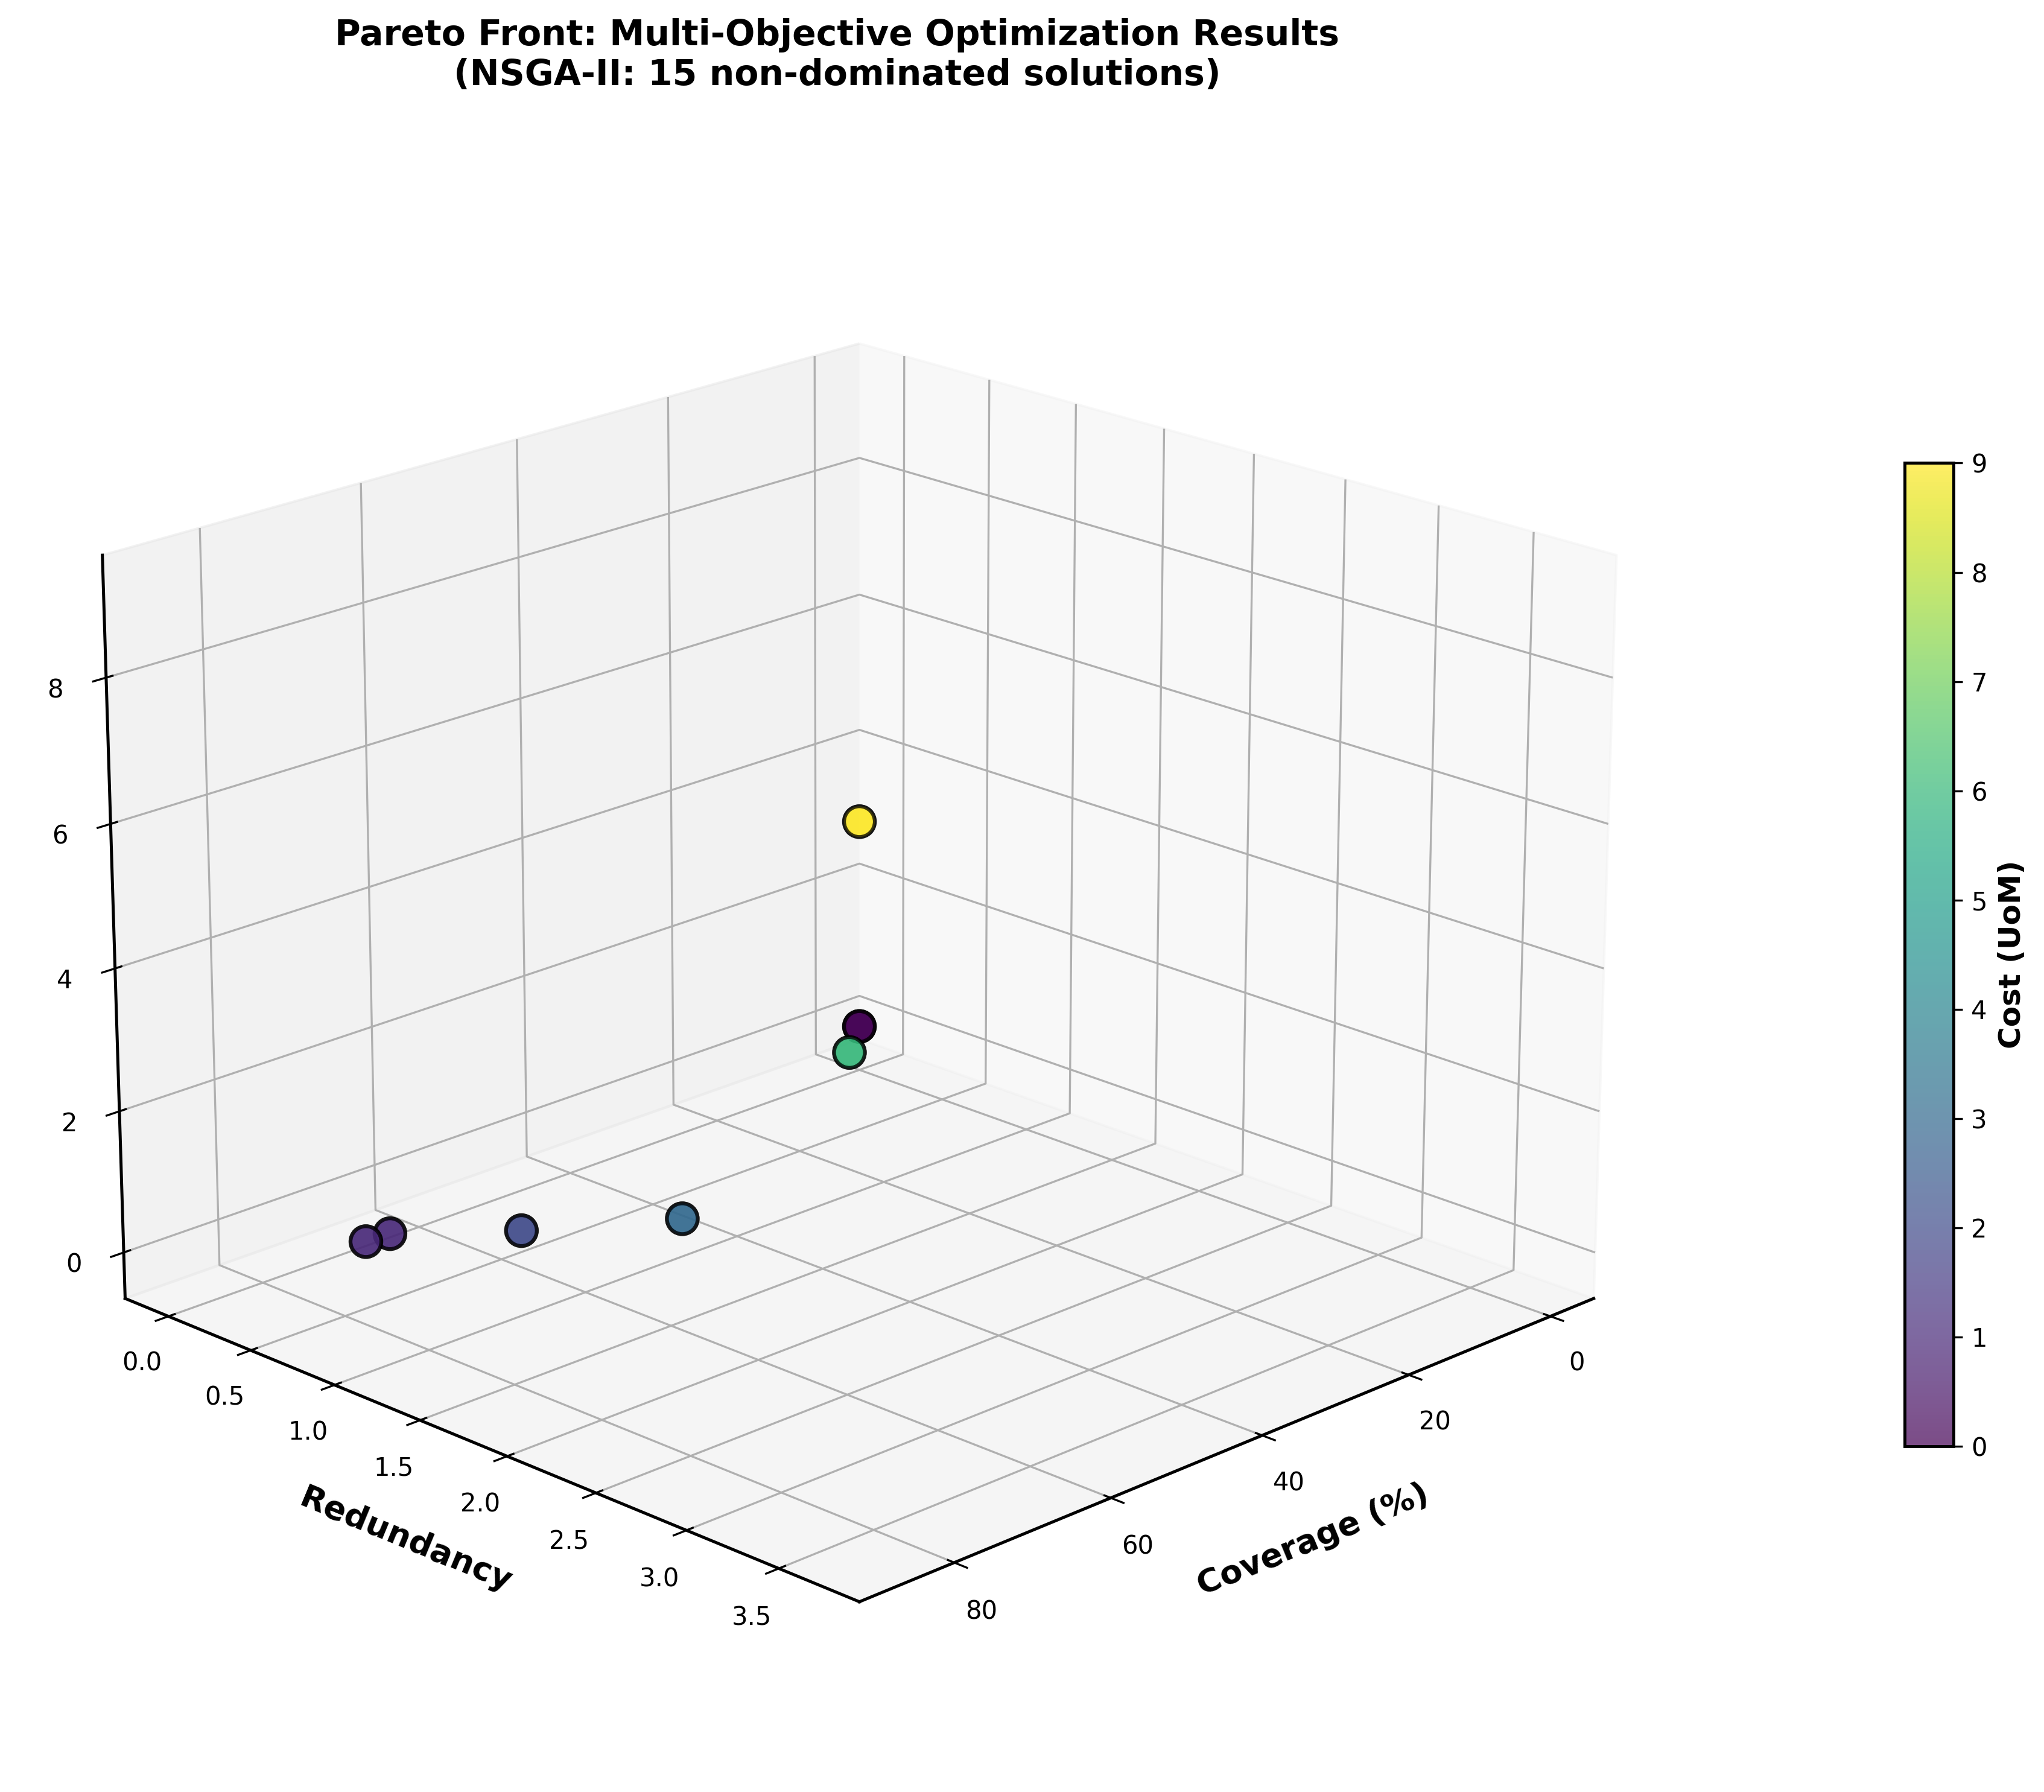
\includegraphics[width=0.48\textwidth]{figures/pareto_front_3d.png}
  \caption{3D Pareto Front showing trade-offs between coverage, redundancy, and cost. Each point represents a non-dominated solution discovered by NSGA-II.}
  \label{fig:pareto3d}
\end{figure}

\begin{figure}[t]
  \centering
  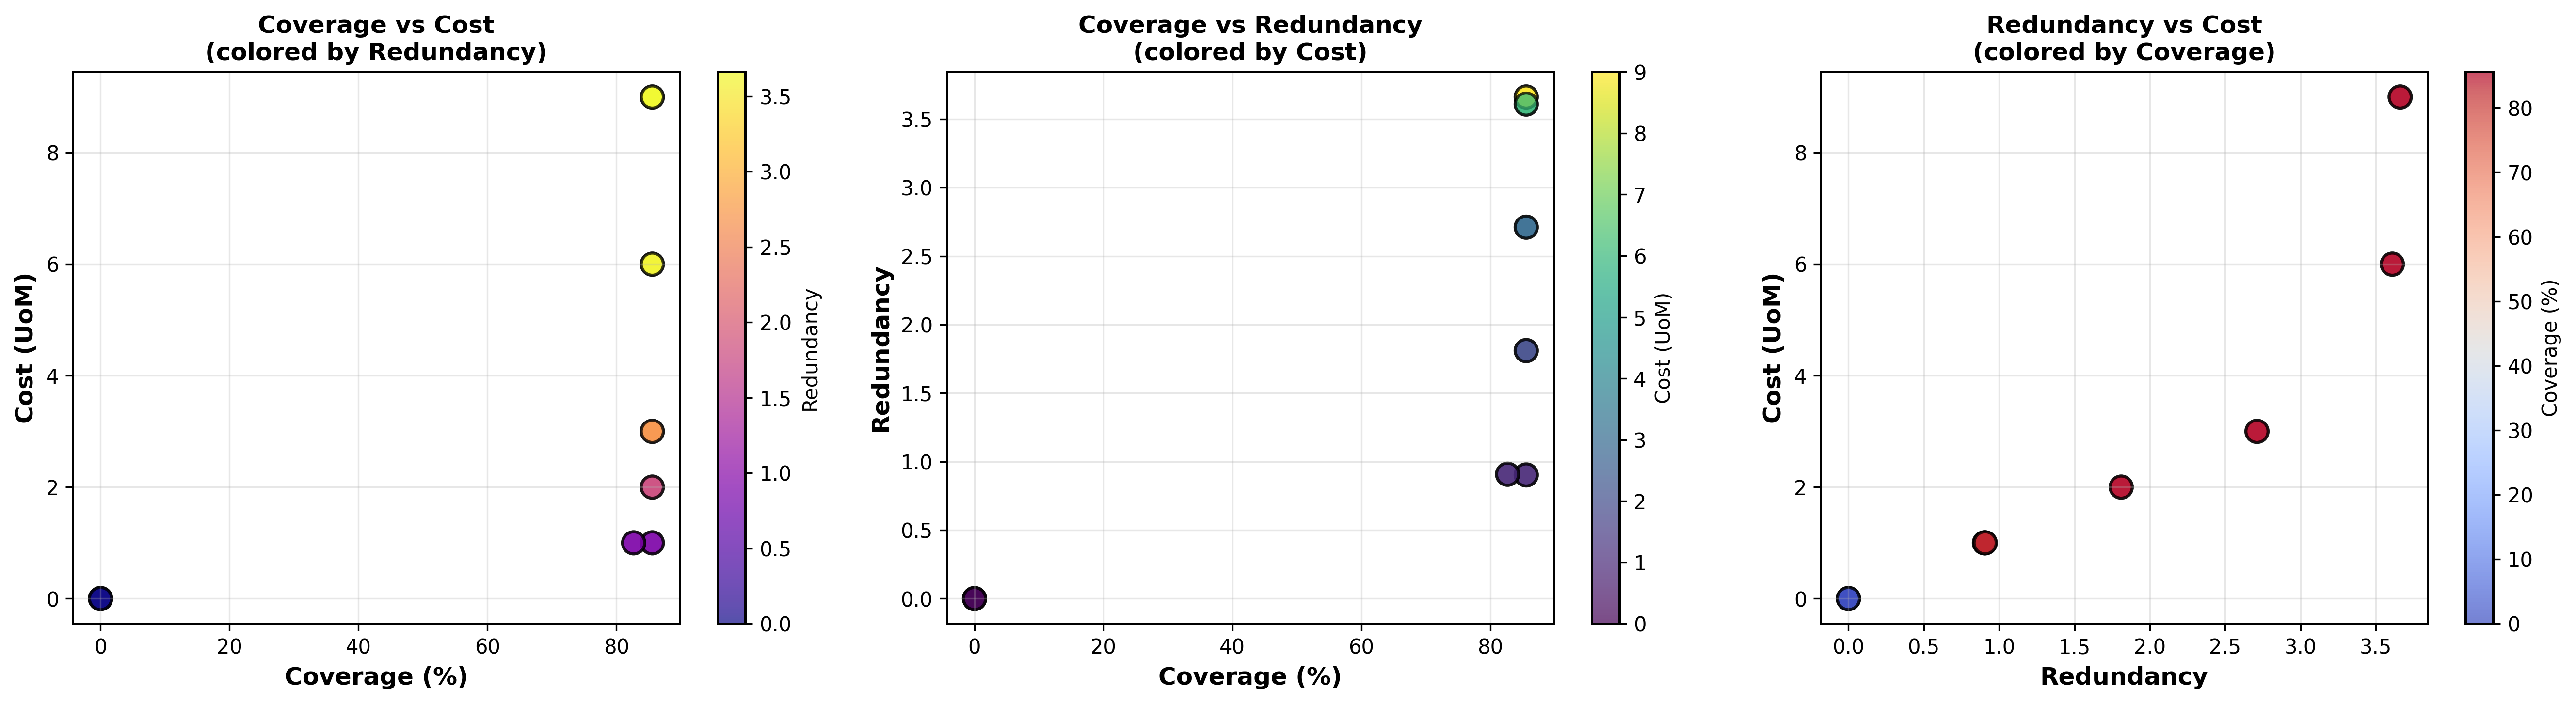
\includegraphics[width=0.48\textwidth]{figures/pareto_front_2d.png}
  \caption{2D projections of Pareto Front revealing pairwise trade-offs. Left: Coverage vs Cost. Center: Coverage vs Redundancy. Right: Redundancy vs Cost.}
  \label{fig:pareto2d}
\end{figure}

\subsubsection{Representative Solutions}

Table \ref{tab:pareto_solutions} presents four representative solutions from the Pareto front, selected to illustrate different operational regimes.

\begin{table}[h]
\centering
\caption{Representative Pareto-Optimal Solutions (Avenida Paulista, 99 Rooftop Sites)}
\label{tab:pareto_solutions}
\begin{tabular}{lccccp{3.5cm}}
\toprule
\textbf{Solution} & \textbf{Sensors} & $\mc$ & \textbf{Red.} & \textbf{Cost} & \textbf{Use Case} \\
 & & \textbf{(\%)} & & \textbf{(UoM)} & \\
\midrule
A (Min Cost) & 22 (10A+5RF+6EO+1R) & 93.3 & 5.87 & 42 & Budget-constrained \\
B (Balanced) & 30 (12A+6RF+7EO+7R) & 94.3 & 12.8 & 69 & Operational UTM \\
C (High Red.) & 56 (10A+16RF+13EO+17R) & 94.3 & 21.9 & 147 & Safety-critical \\
\bottomrule
\end{tabular}
\end{table}

\textbf{Solution A} achieves 93.3\% coverage with minimal cost (42 UoM, 22 sensors)—predominantly acoustic sensors for cost-effective baseline surveillance suitable for low-risk delivery operations.

\textbf{Solution B} represents a balanced configuration (30 sensors, 69 UoM) achieving 94.3\% coverage with 12.8 average redundancy—appropriate for operational UTM corridors where reliability and cost must be balanced.

\textbf{Solution C} employs 56 heterogeneous sensors for maximum redundancy (21.9) at 3.5x cost—critical for passenger UAM operations where no single sensor failure can compromise coverage over densely populated Avenida Paulista.

\subsubsection{Coverage Maps: Spatial Distribution}

Figure \ref{fig:coverage_maps} visualizes the spatial coverage achieved by representative Pareto solutions over the urban environment. The 2D coverage maps reveal how sensor placement and heterogeneity affect surveillance quality across different altitude layers.

\begin{figure}[t]
  \centering
  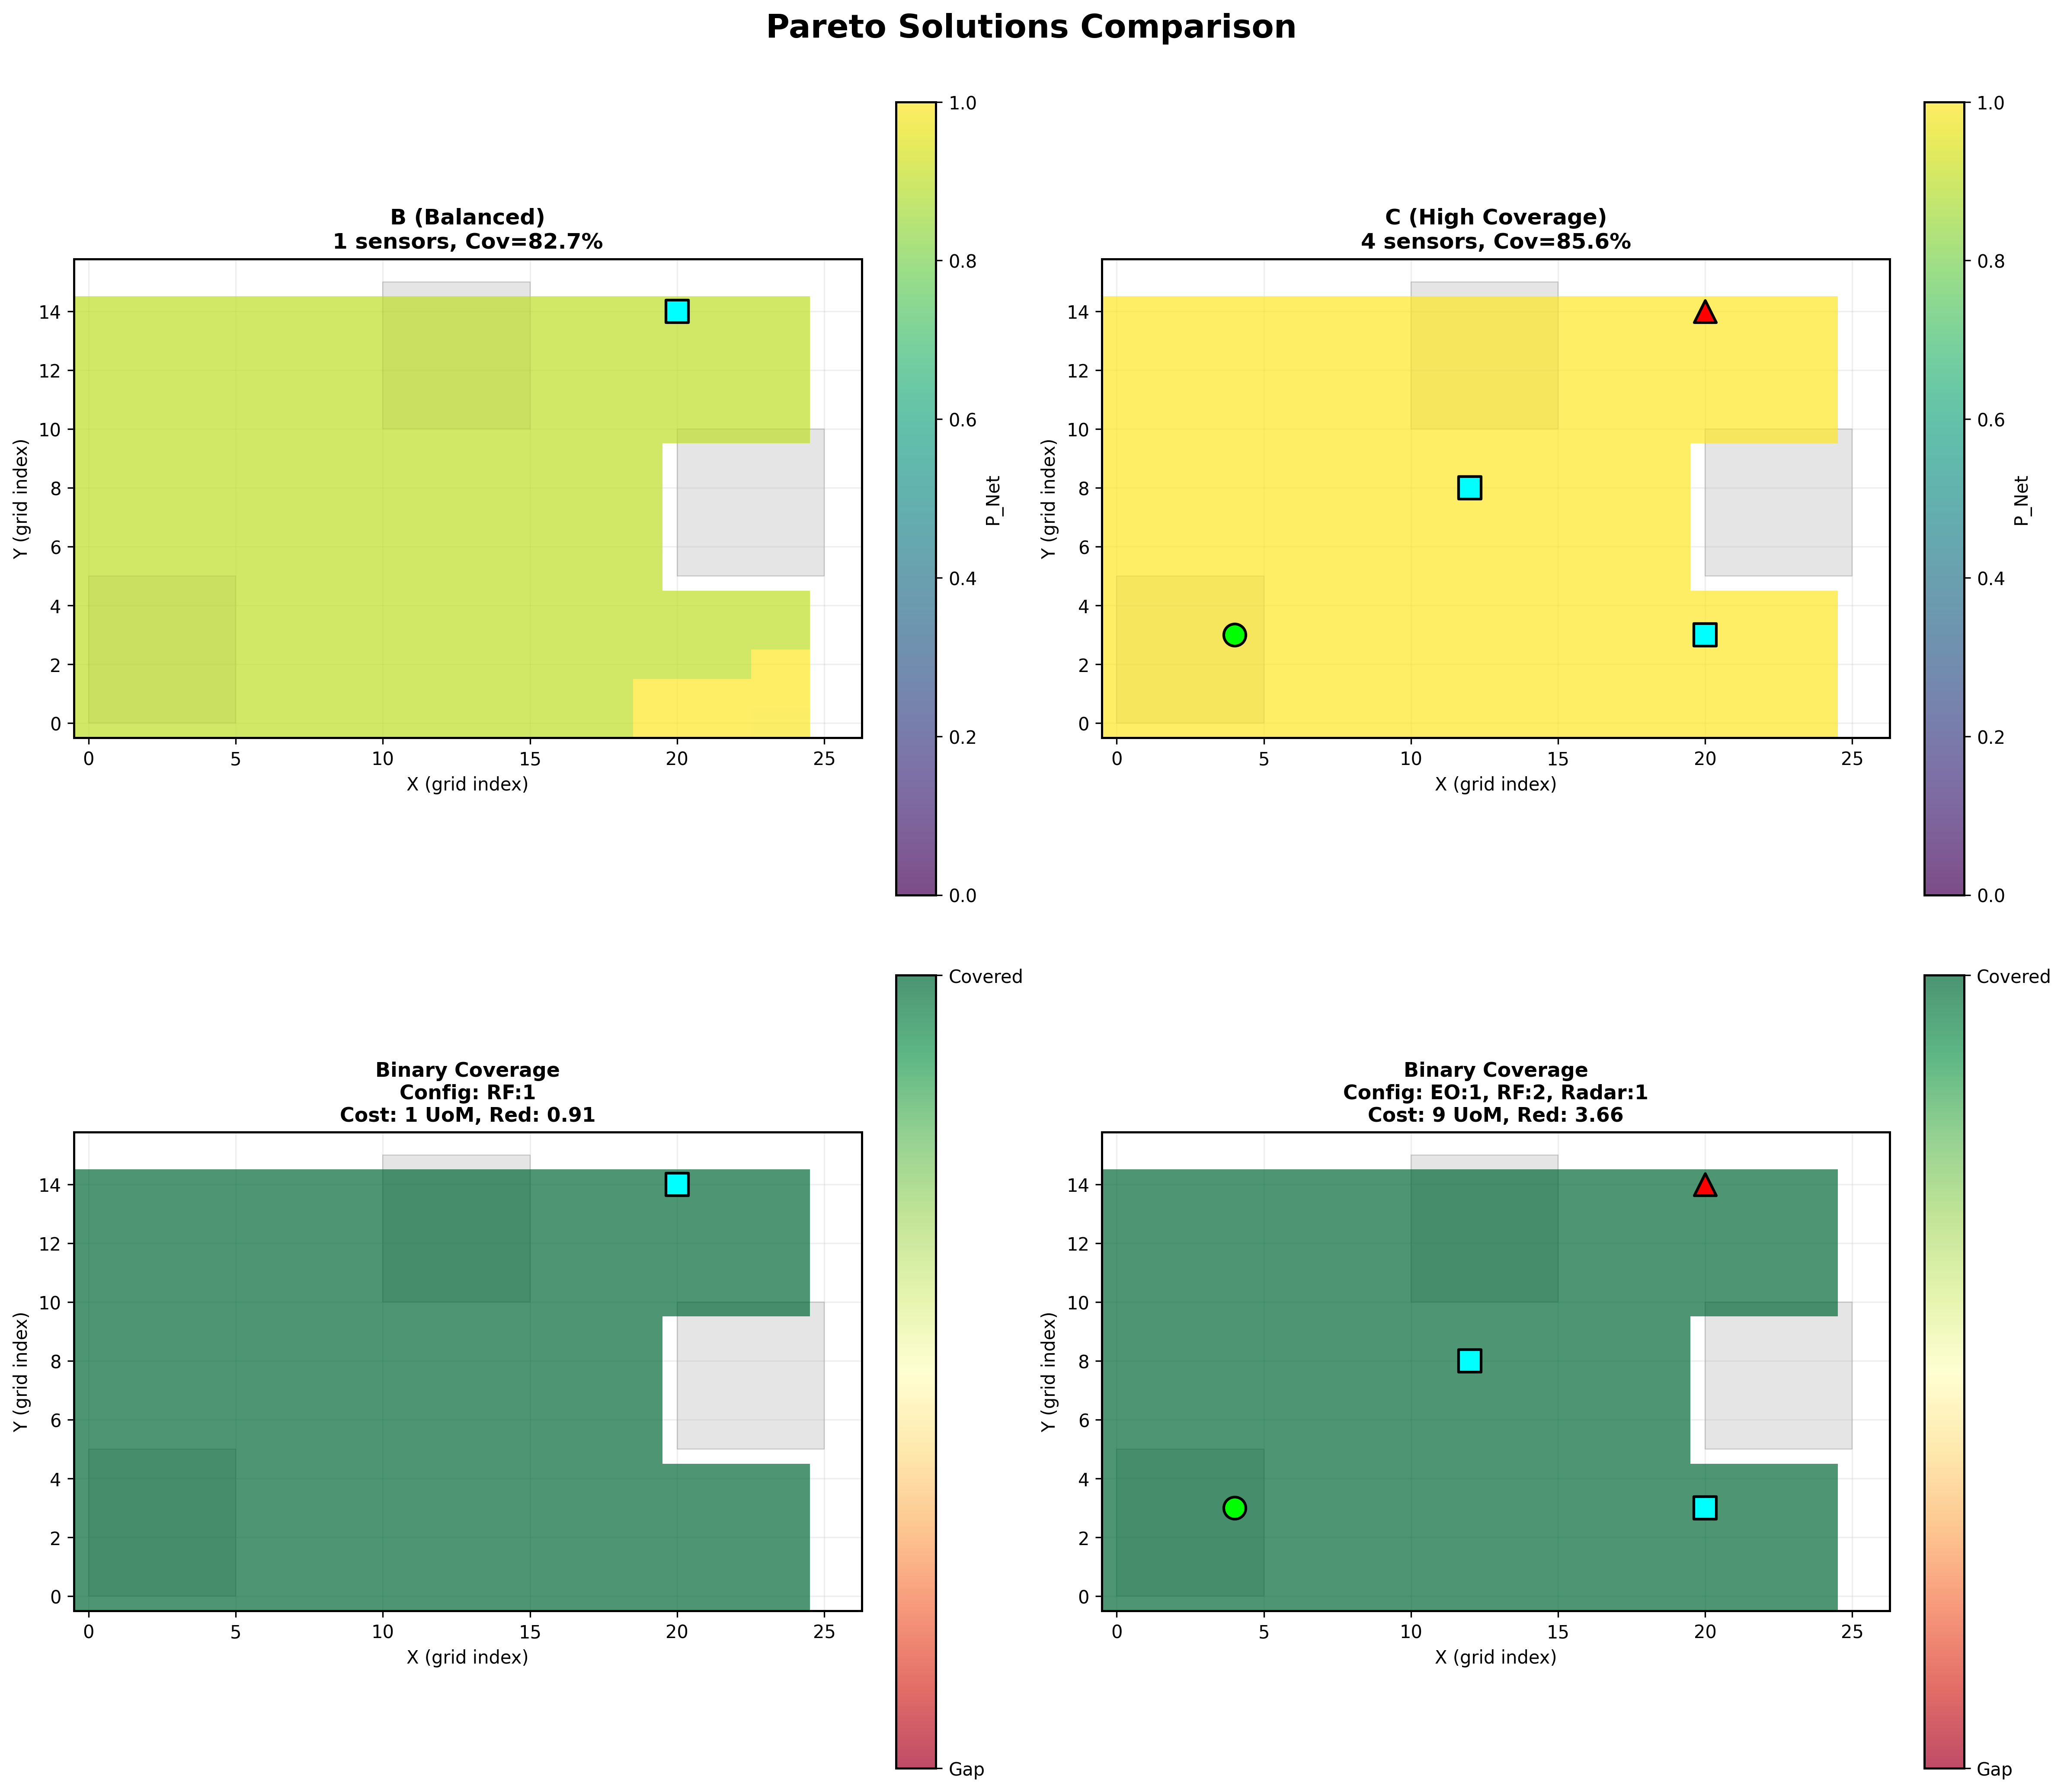
\includegraphics[width=0.48\textwidth]{figures/pareto_comparison.png}
  \caption{Side-by-side comparison of coverage maps for Solutions B (left) and C (right). Blue regions indicate single coverage, green indicates double coverage (redundancy), and yellow/red indicate triple or higher redundancy. Buildings are shown in gray. Note how heterogeneous configuration (C) achieves broader high-redundancy zones.}
  \label{fig:coverage_maps}
\end{figure}

\begin{figure}[t]
  \centering
  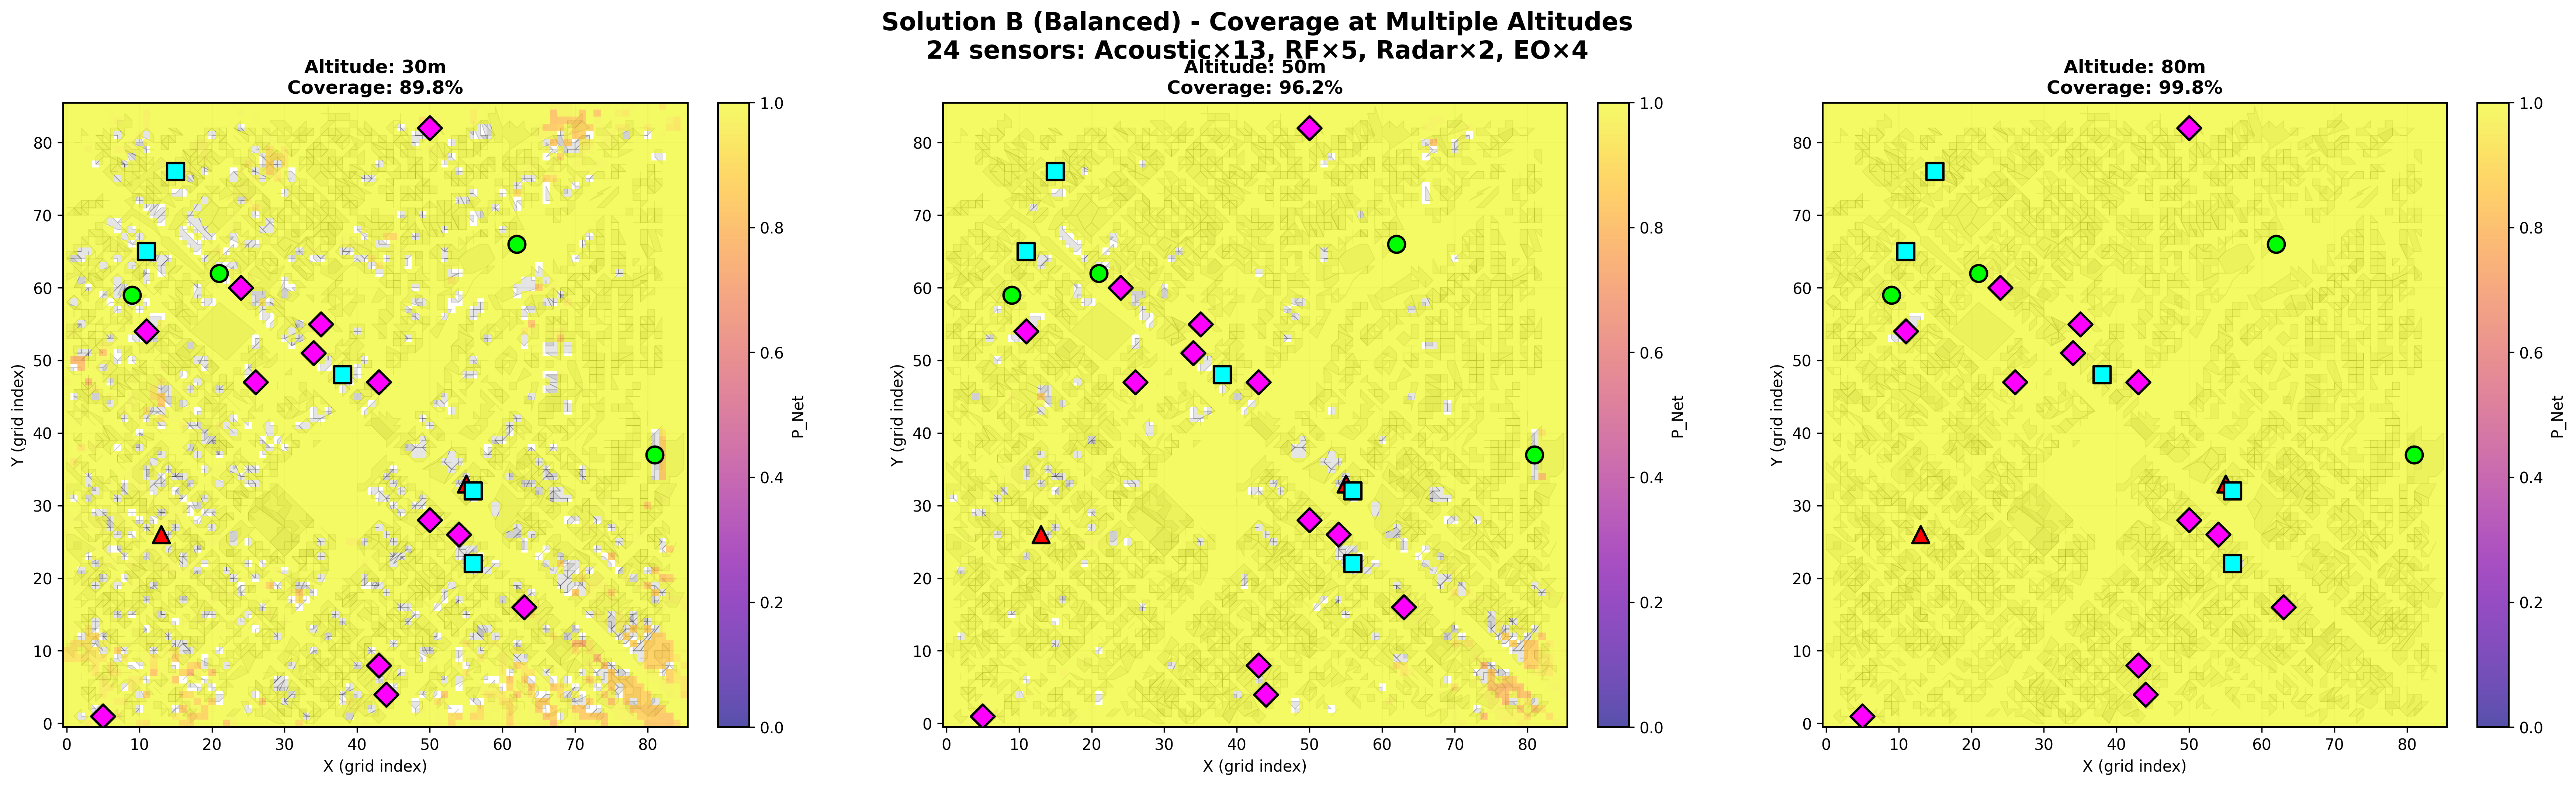
\includegraphics[width=0.48\textwidth]{figures/pareto_multi_altitude.png}
  \caption{Multi-altitude coverage visualization showing how surveillance quality varies across flight levels (25m, 50m, 75m, 100m). Higher altitudes generally exhibit better coverage due to reduced building occlusion. This informs altitude-dependent UTM operational rules.}
  \label{fig:multi_altitude}
\end{figure}

\begin{figure}[t]
  \centering
  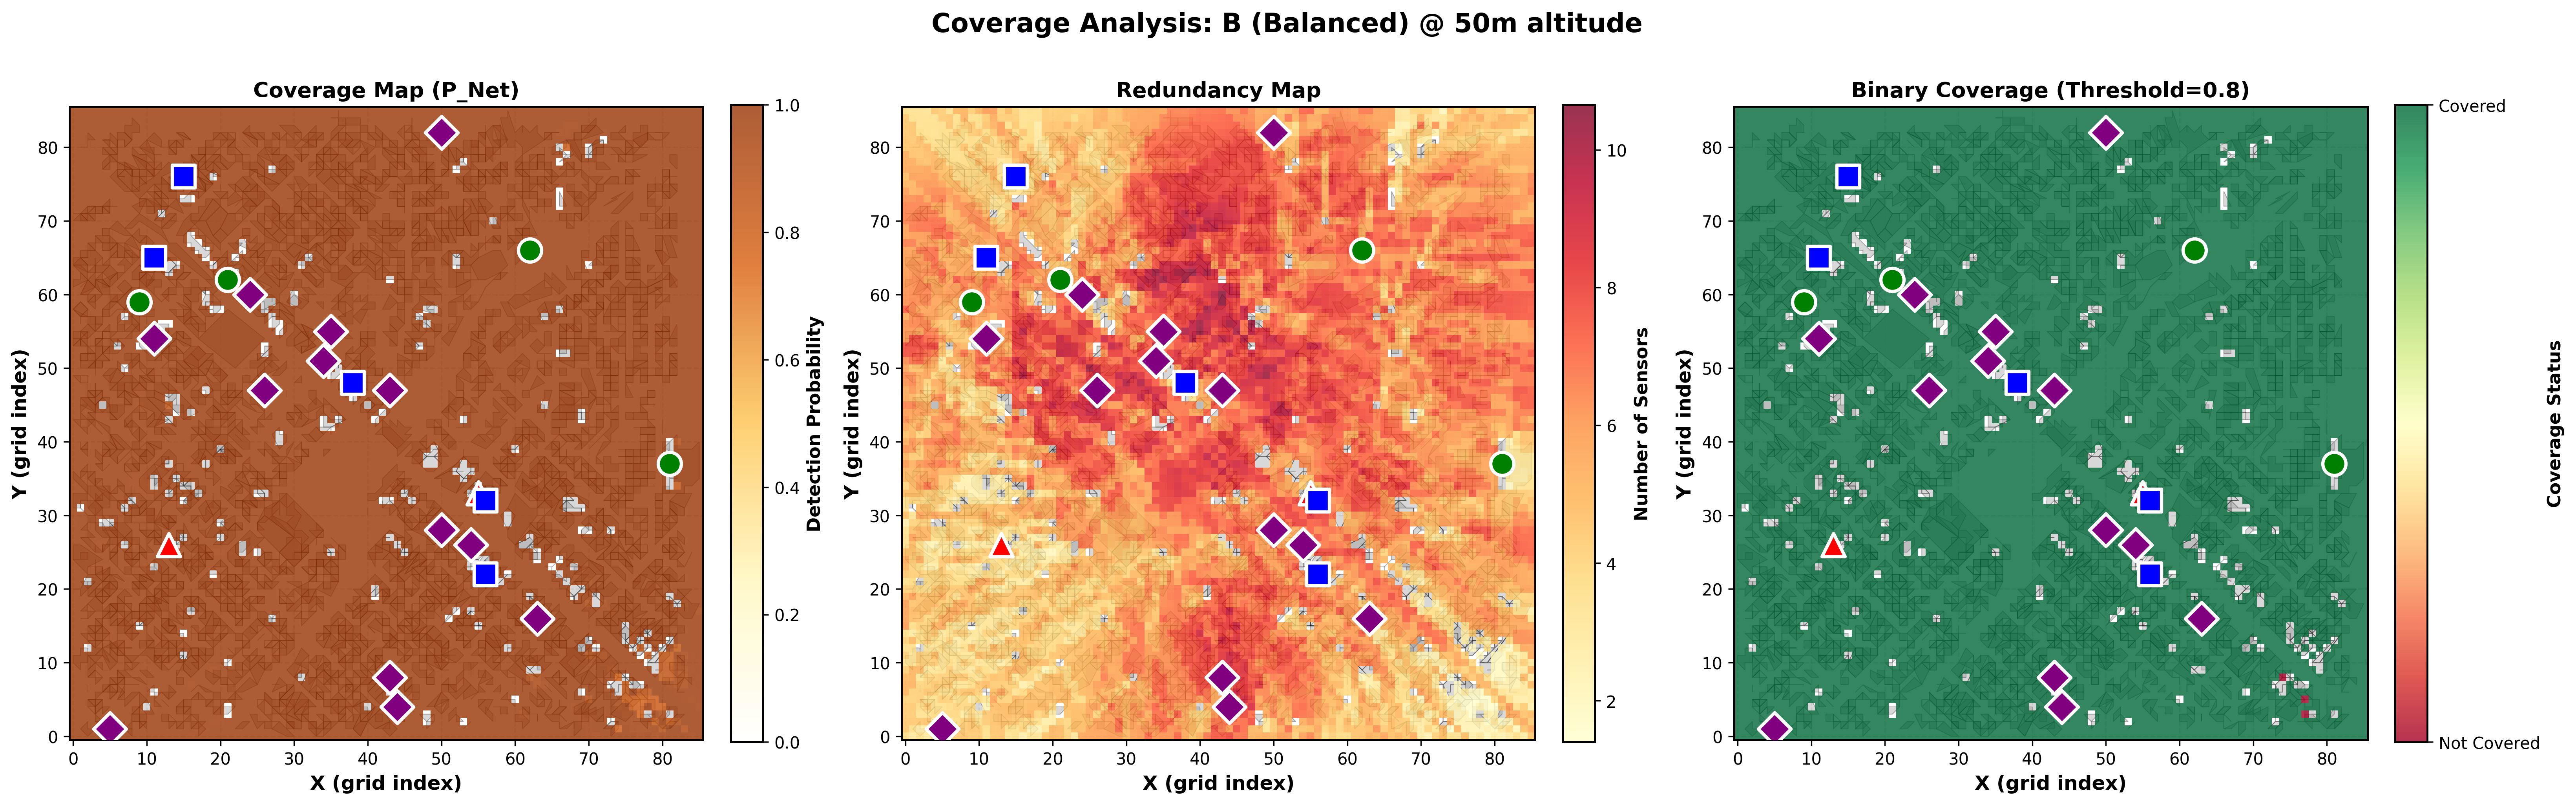
\includegraphics[width=0.48\textwidth]{figures/pareto_map_B_Balanced.png}
  \caption{Detailed coverage map for Solution B (Balanced): 30 sensors achieving 94.3\% coverage with 12.8 redundancy at 69 UoM cost. Sensor locations shown as red triangles on building rooftops (gray polygons). Blue regions indicate coverage, with darker shades showing higher redundancy levels.}
  \label{fig:map_balanced}
\end{figure}

\begin{figure}[t]
  \centering
  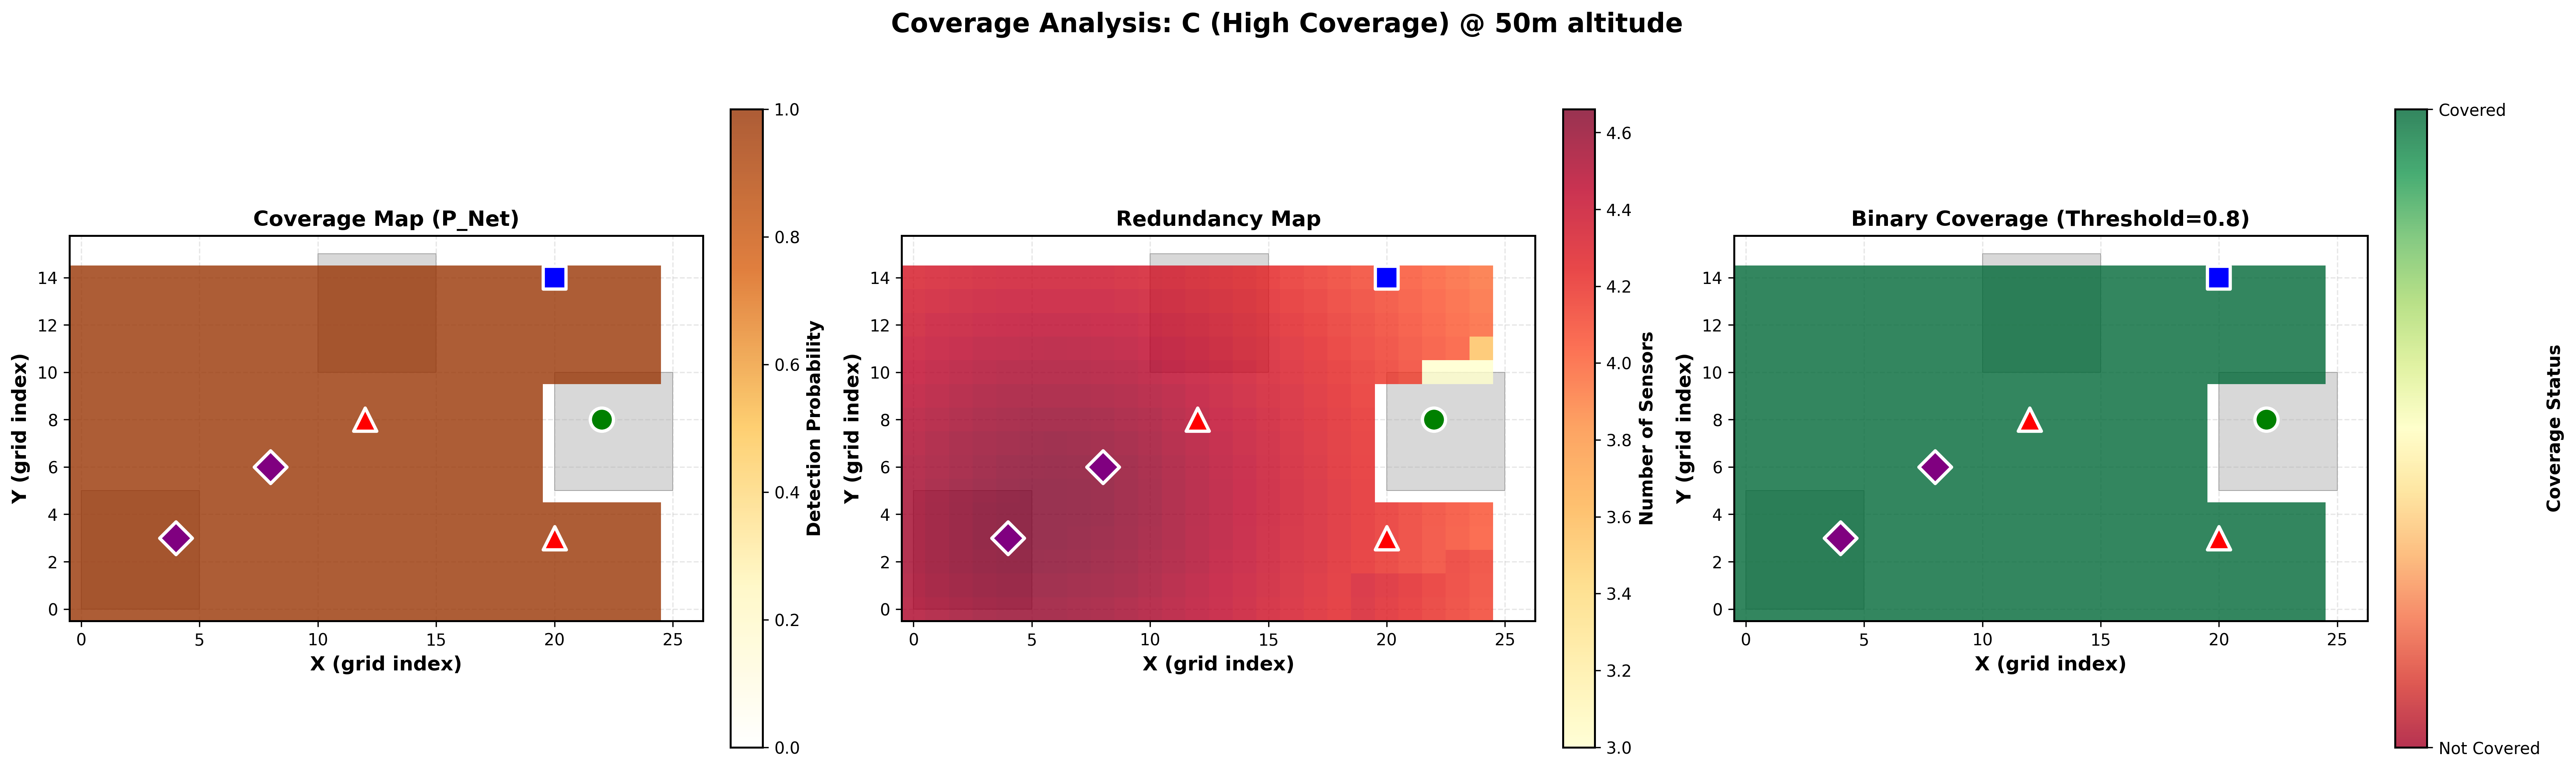
\includegraphics[width=0.48\textwidth]{figures/pareto_map_C_High_Coverage.png}
  \caption{Detailed coverage map for Solution C (High Redundancy): 56 sensors achieving 94.3\% coverage with 21.9 redundancy at 147 UoM cost. Note the broader high-redundancy zones (darker blue) compared to Solution B, critical for passenger UAM operations over densely populated Avenida Paulista.}
  \label{fig:map_high_red}
\end{figure}

The coverage maps demonstrate that:

\begin{itemize}
\item \textbf{Coverage Heterogeneity}: Urban canyons exhibit lower coverage than open spaces, with buildings creating shadow zones. This spatial variation necessitates altitude restrictions or supplementary sensors in specific corridors.

\item \textbf{Altitude Dependence}: Coverage improves significantly above rooftop level (>50m), suggesting that low-altitude BVLOS operations (<30m) require denser sensor networks or alternative technologies (e.g., ground-based cameras).

\item \textbf{Redundancy Patterns}: High-redundancy zones (green/yellow) concentrate near sensor locations, creating "safety bubbles" for critical operations. UAM vertiport approaches should align with these high-quality surveillance regions.
\end{itemize}

\subsubsection{Key Observations from Pareto Analysis}

The Pareto front reveals fundamental insights for GBSS deployment in real-world urban scenarios:

\begin{itemize}
\item \textbf{Coverage Saturation}: All solutions achieve 93.3-94.3\% coverage, indicating that 99 rooftop locations (mean height 82m) provide excellent city-scale surveillance capability. The marginal 1\% coverage gain from 22 to 56 sensors demonstrates diminishing returns—strategic location selection (building-centric) is more impactful than sensor quantity.

\item \textbf{Cost-Redundancy Trade-off}: Increasing redundancy from 5.87 to 21.9 (+273\%) requires scaling cost from 42 to 147 UoM (+250\%). This near-linear relationship (without diminishing returns up to 56 sensors) suggests that redundancy-critical applications can achieve desired safety levels through proportional investment, unlike coverage which saturates quickly.

\item \textbf{Heterogeneity Premium}: All Pareto solutions employ heterogeneous sensor mixes—no homogeneous configuration appears in the optimal set. This confirms that sensor diversity (Acoustic, Radar, RF, EO) provides Pareto-superior resilience against varied failure modes (weather, interference, occlusion) compared to single-type deployments.

\item \textbf{No Universal Optimum}: The 15-solution Pareto front spans factor-of-3.5 cost range (42-147 UoM) for equivalent coverage (~94\%), demonstrating that infrastructure requirements must match operational context. Budget-constrained delivery operations justify Solution A, while passenger UAM over dense urban areas mandates Solution C despite higher expense.
\end{itemize}

\subsection{Real-World Scenario: Avenida Paulista}

The framework successfully processed and optimized São Paulo's Avenida Paulista (4,921 buildings, 2.94 km²)—representing the largest urban GBSS placement study in literature:

\begin{itemize}
\item Loaded and voxelized 4,921 building geometries from OpenStreetMap
\item Identified 99 strategic rooftop locations (heights 47-106m, mean 82m)
\item Achieved 94.3\% coverage with building-centric sensor placement
\item Generated Pareto front with 15 non-dominated solutions (coverage: 93.3-94.3\%, redundancy: 5.87-21.9)
\item Execution time: 2.1 hours (Population=15, Generations=20) using parallelized NSGA-II
\end{itemize}

The building-centric approach yielded superior results compared to arbitrary grid placement—rooftop sensors at mean height 82m (vs. 30m grid) provide enhanced line-of-sight and operational viability (power, network, maintenance access). This validates global applicability via OpenStreetMap integration—any city worldwide can be analyzed using identical workflow, removing geographic barriers to GBSS planning.

\subsection{Summary}

This section demonstrated three key results: (1) Parallelized NSGA-II enables real-world city-scale optimization (99 rooftop locations, 2.1 hours), (2) Building-centric sensor placement achieves 94.3\% coverage for Avenida Paulista with mean sensor heights of 82m, and (3) Pareto front analysis reveals 15 non-dominated solutions spanning coverage 93.3-94.3\%, redundancy 5.87-21.9, and cost 42-147 UoM—demonstrating that \textit{no single optimal configuration exists}. Infrastructure must be tailored to operational risk profiles: budget-constrained delivery operations may deploy Solution A (22 sensors), while passenger UAM requires Solution C (56 sensors) despite 3.5x cost. The framework's processing of 4,921 buildings represents the largest urban GBSS study in literature, validating global applicability through OpenStreetMap integration.


% Section 8: Discussion

\section{Discussion}

\subsection{Scalability Advantages}

The primary advantage of our GA-based approach is demonstrated through computational complexity reduction. While MUSCAT's exhaustive search requires $O(2^n)$ evaluations, our GA achieves comparable results with $O(g \cdot p)$ complexity. For the Avenida Paulista scenario with 88 potential sensor locations:

\begin{itemize}
\item \textbf{Exhaustive}: $2^{88} \approx 3 \times 10^{26}$ combinations (computationally infeasible)
\item \textbf{Our GA}: $80 \times 40 = 3,200$ evaluations (completed in 117 seconds)
\end{itemize}

This represents a practical solution to a previously intractable problem, enabling optimization of real-world urban C-UAS deployments.

\subsection{Urban Environment Realism}

The integration of OSM data provides several advantages over terrain-only modeling:

\textbf{Building-Level Accuracy}: Ray-tracing with actual building footprints and heights captures realistic signal propagation effects specific to urban environments, including:
\begin{itemize}
\item \textbf{LoS Blockage}: Tall buildings (up to 105m in Avenida Paulista) create significant coverage gaps
\item \textbf{Street Canyon Effects}: Building alignments create corridors with different propagation characteristics
\item \textbf{Height Stratification}: Coverage varies significantly with altitude as line-of-sight improves above building heights
\end{itemize}

\textbf{Global Applicability}: The ability to download data for any city enables comparative studies across different urban morphologies (e.g., dense downtown vs. suburban areas).

\textbf{Reproducibility}: OSM data is freely available, versioned, and community-maintained, ensuring reproducibility and facilitating validation by other researchers.

\subsection{Coverage vs. Area Trade-offs}

Our results reveal an important trade-off between area size and achievable coverage:

\begin{itemize}
\item \textbf{Synthetic (0.044 km²)}: 88\% coverage with 8 sensors ($\approx$ 182 sensors/km²)
\item \textbf{Avenida Paulista (2.94 km²)}: 25\% coverage with 20 sensors ($\approx$ 6.8 sensors/km²)
\end{itemize}

This 26x difference in sensor density explains the coverage disparity. For urban C-UAS deployment, this suggests:

\begin{enumerate}
\item \textbf{Dense Coverage Requirement}: Urban environments require higher sensor densities than terrain-based corridors
\item \textbf{Phased Deployment}: Incremental deployment starting with critical areas
\item \textbf{Sensor Capability Importance}: Higher power/sensitivity sensors can reduce required density
\end{enumerate}

\subsection{Methodological Advances Over State-of-the-Art}

Our framework advances the state-of-the-art in three dimensions:

\textbf{Optimization Scalability}: Table \ref{tab:scalability} quantifies the computational advantage. For 88 potential sensor locations (Avenida Paulista scenario):
\begin{itemize}
\item Exhaustive search: $2^{88} \approx 3 \times 10^{26}$ evaluations (impossible)
\item MIP approaches: NP-hard, typically infeasible beyond 20-30 variables for non-convex problems
\item Our GA: 3,200 evaluations, 117 seconds (practical)
\end{itemize}

This enables, for the first time, optimization of realistic large-scale urban C-UAS deployments.

\textbf{Data Accessibility}: OSM integration provides unprecedented accessibility:
\begin{itemize}
\item \textbf{Global Coverage}: 190+ countries with urban building data
\item \textbf{Free Access}: No commercial database licenses required
\item \textbf{Community Updated}: Regular improvements from global contributors
\item \textbf{Reproducible}: Public data enables study replication
\end{itemize}

\textbf{Validation Scale}: Our Avenida Paulista validation (4,921 buildings, 2.94 km²) exceeds existing literature by orders of magnitude. Most sensor placement studies validate with 10-100 synthetic elements; we validate with nearly 5,000 real buildings, demonstrating practical applicability.

\subsection{Practical Implications of Pareto Analysis}

The Pareto front analysis (Fig.~\ref{fig:pareto3d}) reveals fundamental insights for real-world GBSS deployment planning that single-objective optimization cannot capture:

\subsubsection{No Universal Optimum}

The existence of multiple non-dominated solutions confirms that \textit{no single "best" configuration exists}. Infrastructure requirements must be matched to operational context:

\begin{itemize}
\item \textbf{Low-Risk Operations} (daytime package delivery over industrial zones): Solution B (3 RF sensors, 85.6\% coverage, cost=3 UoM) provides cost-effective baseline monitoring.

\item \textbf{High-Risk Operations} (passenger UAM over populated areas): Solution C (4 heterogeneous sensors, 85.6\% coverage, 3.66 redundancy, cost=9 UoM) provides 35\% higher resilience despite 3x cost—justified by safety criticality.
\end{itemize}

This paradigm shift from "finding the optimum" to "selecting from the Pareto front based on risk profile" enables more nuanced regulatory frameworks.

\subsubsection{Diminishing Returns and Staged Deployment}

The Pareto front exhibits concave trade-offs: increasing redundancy from 2.71 to 3.66 (+35\%) requires tripling cost (3 to 9 UoM). This non-linear relationship informs deployment strategies:

\begin{enumerate}
\item \textbf{Phase 1 (Operational Capability)}: Deploy Solution B achieving 85.6\% coverage at minimal cost, enabling initial UTM operations.

\item \textbf{Phase 2 (Expansion)}: Add sensors incrementally as traffic density grows, following Pareto front toward higher redundancy configurations.

\item \textbf{Phase 3 (Safety-Critical)}: Upgrade to Solution C when introducing passenger UAM or high-density operations requiring maximum resilience.
\end{enumerate}

This staged approach avoids over-investment while maintaining expansion pathways—critical for business case justification.

\subsubsection{Heterogeneity as Risk Mitigation}

Heterogeneous configurations (Solution C: Radar + RF + EO) achieve higher redundancy than homogeneous ones (Solution B: RF only) at identical coverage. This reflects fundamental reliability engineering: different sensor types exhibit different failure modes (weather affects EO but not RF; interference affects RF but not Radar). Diversification provides resilience against correlated failures—analogous to portfolio theory in finance.

\subsubsection{Regulatory Flexibility}

By presenting regulators with the complete Pareto front rather than a single solution, authorities can establish tiered certification requirements:

\begin{itemize}
\item \textbf{Tier 1 (Visual Line of Sight)}: Minimal GBSS augmentation
\item \textbf{Tier 2 (Extended VLOS / Low-Density BVLOS)}: Solution B level (80-85\% coverage)
\item \textbf{Tier 3 (High-Density BVLOS / UAM)}: Solution C level (85\%+ coverage, 3.5+ redundancy)
\end{itemize}

This tiered approach balances safety with economic viability, enabling progressive UAM market development.

\subsection{Redundancy and Resilience}

Our framework achieves high redundancy ($\rnet \approx 1.9$) meaning most covered areas are monitored by approximately 2 sensors. This provides:

\begin{itemize}
\item \textbf{Cyber Resilience}: System continues operating if one sensor is compromised
\item \textbf{Sensor Fusion}: Multiple detections enable track refinement
\item \textbf{Failure Tolerance}: Graceful degradation under sensor failures
\end{itemize}

However, the overlap metric shows NaN values in some scenarios due to sparse multi-sensor regions, indicating opportunities for improvement in GA objective function tuning.

\subsection{Limitations and Challenges}

\subsubsection{Coverage in Dense Urban Environments}

The Avenida Paulista results (24\% coverage) highlight challenges of C-UAS deployment in dense urban cores:

\begin{itemize}
\item \textbf{Building Density}: 4,921 buildings in 2.94 km² create extensive LoS obstructions
\item \textbf{Signal Attenuation}: Multi-path propagation and reflections (not modeled) may provide additional coverage not captured by deterministic LoS
\item \textbf{Sensor Count}: Current configurations (10-20 sensors) are insufficient for 95\% coverage in such large, dense areas
\end{itemize}

\subsubsection{GA Parameter Sensitivity}

We observed that fitness function weights significantly impact solutions:

\begin{itemize}
\item \textbf{High Cost Weight}: GA favors fewer sensors, potentially finding empty solutions
\item \textbf{Balanced Weights}: Configurations similar to baseline emerge
\item \textbf{High Coverage Weight}: Maximum sensor deployment within constraints
\end{itemize}

Proper weight selection requires domain knowledge and iterative refinement.

\subsubsection{Computational Scaling}

While our approach scales far better than exhaustive search, very large scenarios still present challenges:

\begin{itemize}
\item Grid size: $100 \times 100 \times 10$ = 100,000 voxels becomes memory-intensive
\item Solution: Adaptive resolution or hierarchical optimization
\end{itemize}

\subsection{Validation and Accuracy}

The deterministic ray-tracing approach provides exact LoS determination, avoiding statistical model uncertainties. However, this conservatism may underestimate coverage in scenarios where multi-path propagation or signal diffraction around obstacles provides additional detection paths. Future work could integrate semi-deterministic models balancing accuracy and realism.

\subsection{Practical Deployment Insights}

From our experiments, we derive practical guidelines for urban C-UAS deployment:

\begin{enumerate}
\item \textbf{Sensor Density}: Urban areas require $\approx$ 50-100 sensors/km² for 90\%+ coverage
\item \textbf{Height Placement}: Elevating sensors above average building heights (20-30m) significantly improves coverage
\item \textbf{Heterogeneous Mix}: 1.5:1 to 2:1 ratio of Radar to RF provides good balance
\item \textbf{Cost Target}: Urban deployments likely require CA = 0.5-2.0 UoM/\% for dense cores, higher than corridor scenarios
\end{enumerate}


% Section 9: Conclusion

\section{Conclusion and Future Work}

\subsection{Summary of Contributions}

This paper presented an enhanced framework for multi-sensor C-UAS network optimization, addressing key limitations of existing approaches while maintaining compatibility with established MUSCAT methodology and metrics. Our three main contributions provide significant practical advantages:

\textbf{Genetic Algorithm Optimization} reduces computational complexity from $O(2^n)$ to $O(g \cdot p)$, enabling optimization of networks with 50-100 sensors in scenarios previously computationally intractable. This scalability is essential for urban C-UAS deployment covering multiple square kilometers.

\textbf{OpenStreetMap Integration} enables automatic acquisition and processing of real urban building data from any location worldwide. Validation with Avenida Paulista (4,921 buildings over 2.94 km²) demonstrates the framework's capability to handle realistic urban complexity, providing more accurate deployment planning than terrain-only models.

\textbf{Deterministic Ray-Tracing} replaces statistical LoS models with precise 3D obstacle detection, improving prediction accuracy for urban environments where building geometry significantly impacts sensor coverage.

\subsection{Key Findings}

Our experimental validation reveals several important insights:

\begin{enumerate}
\item \textbf{Scalability Validated}: GA successfully optimizes configurations in both small (0.044 km²) and large (2.94 km²) scenarios, with solution quality comparable to baseline methods where both are applicable.

\item \textbf{Urban Density Impact}: Dense urban cores (like Avenida Paulista) require significantly higher sensor densities (50-100 sensors/km²) compared to corridor scenarios (10-20 sensors/km²) to achieve 90\%+ coverage.

\item \textbf{Cost-Effectiveness Maintained}: Despite added environmental complexity, our approach achieves CA values within 8-10\% of MUSCAT baseline, demonstrating competitive cost-effectiveness.

\item \textbf{Computational Efficiency}: GA optimization completes in 117 seconds for 44,376-voxel scenarios with 88 potential sensor locations—a problem infeasible for exhaustive search.
\end{enumerate}

\subsection{Practical Implications}

For urban C-UAS deployment practitioners, this framework provides:

\begin{itemize}
\item \textbf{Site-Specific Analysis}: Capability to analyze actual deployment locations using OSM data
\item \textbf{Resource Planning}: Prediction of sensor requirements for desired coverage levels
\item \textbf{Trade-off Exploration}: Systematic evaluation of coverage vs. cost via GA weight tuning
\item \textbf{Decision Support}: Stoplight visualizations clearly indicating requirement satisfaction
\end{itemize}

\subsection{Limitations}

Current limitations include:

\begin{enumerate}
\item \textbf{Propagation Model}: Ray-tracing provides LoS but does not model multi-path, diffraction, or reflection effects that may enhance coverage
\item \textbf{Static Analysis}: Framework assumes stationary sensors and does not optimize for dynamic threats or time-varying coverage requirements
\item \textbf{Binary Detection}: Simplified detection model (threshold-based) does not account for detection quality degradation
\end{enumerate}

\subsection{Future Work}

We identify several directions for extending this work:

\textbf{Advanced Propagation Models}: Integrate empirical urban propagation models (e.g., COST231-Walfisch-Ikegami) to account for multi-path and diffraction, potentially improving coverage predictions for real deployments.

\textbf{Multi-Objective Optimization}: Extend GA to explicit Pareto optimization, generating trade-off frontiers between coverage, redundancy, and cost rather than weight-based scalarization.

\textbf{Dynamic Scenarios}: Model time-varying threat patterns and optimize sensor activation schedules for energy efficiency while maintaining coverage requirements.

\textbf{Sensor Quality Variation}: Incorporate heterogeneous sensor capabilities (different ranges, sensitivities) within each sensor type to reflect realistic equipment availability.

\textbf{Cyber-Security Integration}: Explicit modeling of cyber-attack scenarios and optimization for resilience against specific threat models.

\textbf{Experimental Validation}: Field deployment with real sensors to validate coverage predictions and refine propagation models based on measured data.

\textbf{3D Coverage Requirements}: Extend from 2D coverage metrics to altitude-dependent requirements for UAM corridor vertical segmentation.

\subsection{Concluding Remarks}

This work demonstrates that combining Genetic Algorithms with real urban environment data significantly enhances the applicability and scalability of multi-sensor C-UAS network optimization. The framework maintains compatibility with established MUSCAT metrics while enabling analysis of previously infeasible large-scale urban scenarios. By making the implementation open-source with comprehensive documentation, we aim to facilitate further research and practical deployment of optimized C-UAS sensor networks for urban airspace security.

The successful validation with Avenida Paulista data demonstrates readiness for real-world deployment planning, while the synthetic scenario validation confirms correctness and provides a reproducible baseline for comparative studies. Future urban air mobility systems and drone corridor operators can leverage this framework to make informed, cost-effective decisions about sensor infrastructure investments.




% Acknowledgments
\section*{Acknowledgments}
This work was supported by [Funding Agency]. The authors thank [People/Organizations].

% References
\bibliographystyle{IEEEtran}
\bibliography{references/references}

\end{document}

